In this chapter, we analyze the first experiment, that is, the impact of using different scoring techniques in a Blockchain-based Federated Learning system. In this set of experiments, all properties of the system are static, except for the scoring technique, which varies between BlockFlow, Marginal Gain, Multi-KRUM, or none.

\section{Execution Time, Transaction Cost and Latency}

With respect to execution times, we can see on \autoref{tab:metrics_scoring} that every scoring technique gives different results. Since using no scoring technique means that there are less transactions and less computations, it is expected that using no scoring technique would be the fastest. That is observable on \autoref{tab:metrics_scoring}, where it is shown that using no scoring technique is twice as fast as most scoring techniques. The fastest scoring technique is Multi-KRUM, taking around $31$ seconds per round; while both BlockFlow and Marginal Gain are the slowest, taking both around $49$ seconds per round.

\begin{table}[!ht]
\centering
\begin{tabular}{c|c|c|c|c} \hline \hline
                               & None   & BlockFlow & Marginal Gain & Multi-KRUM \\ \hline \hline
E2E Time (m)                   & 18.93  & 40.95     & 41.38         & 26.25      \\ \hline
Mean Round Time (s)            & 22.70  & 49.11     & 49.64         & 31.48      \\ \hline
% Median Round Time (s)          & 21.90  & 49.49     & 43.97         & 31.26      \\ \hline
Mean Transaction Latency (s)   & 1.549  & 1.564     & 1.577         & 1.573      \\ \hline
% Median Transaction Latency (s) & 1.549  & 1.558     & 1.564         & 1.551      \\ \hline
Mean Transaction Cost (Gas)    & 183124 & 339645    & 257686        & 280733     \\ \hline
% Median Transaction Cost (Gas)  & 185198 & 189092    & 188994        & 187152     \\ \hline
\end{tabular}
\caption{Time and Transaction Metrics Per Scoring Technique}
\label{tab:metrics_scoring}
\end{table}

We can notice that BlockFlow and Marginal Gain, not only take the longest, but also take a very similar amount of time. As explained in \autoref{background:scoring}, BlockFlow and Marginal Gain scores are computed by other clients, where the Multi-KRUM is computed by the servers. Since the amount of clients is larger than the amount of servers, there are more devices performing scoring computations. For each scoring submission, there is a transaction. The more transactions there are, the more the system has to wait for the blockchain. In addition, clients are usually devices with less computational power. Wherefore, it is expected that techniques that run on the clients, such as BlockFlow and Marginal Gain, take longer than techniques that run on the servers, such as Multi-KRUM.

On one hand, we can observe that transaction latency is not influenced by the scoring techniques. The transaction latency, as seen before, is mostly influenced by the consensus algorithm, which, in this case, is static across the experiments. On the other hand, transaction costs are much higher when using a scoring technique. Scoring techniques add at least one more transactions per round per device. Since transaction costs work on a "supply and demand" basis, it is expected that the more transactions are required, the higher the cost will be.

\section{Accuracy and Convergence}

\begin{figure}[!ht]
    \centering
    \centering
    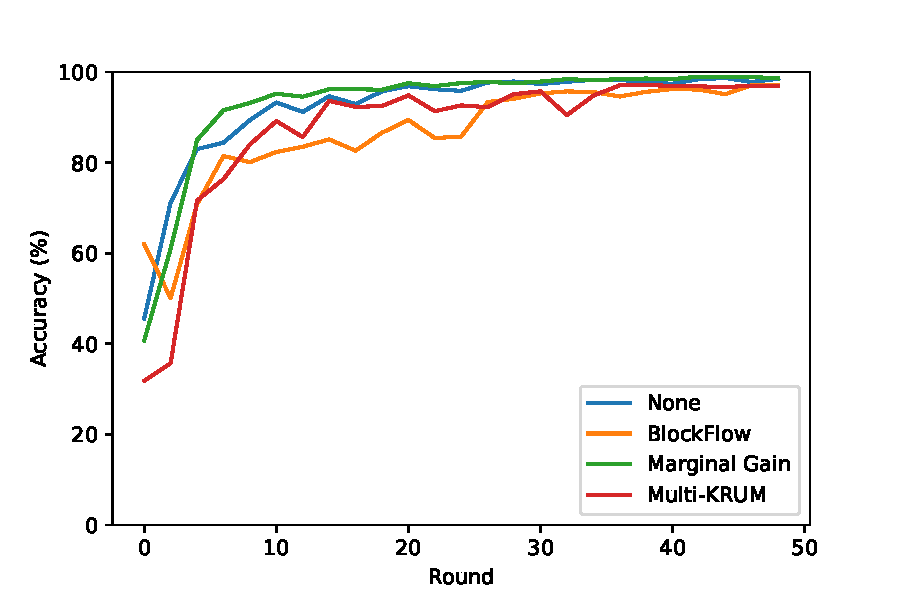
\includegraphics[width=0.7\textwidth]{graphics/04_scoring_accuracy.pdf}
    \caption{Accuracy Per Scoring Technique}
    \label{fig:accuracy_scoring}
\end{figure}

When comparing the accuracy across the different scoring techniques, we can see on \autoref{fig:accuracy_scoring} that all techniques reached a very high accuracy of above $97\%$. However, some techniques reach higher values faster than others, that is, some converge faster than others.

As we can see, Marginal Gain converges the fastest, followed by no scoring technique, then Multi-KRUM and lastly the BlockFlow technique. 

As we can see, Marginal Gain converges the fastest, followed by no scoring technique, then Multi-KRUM and lastly the BlockFlow technique. Both Marginal Gain and Multi-KRUM have a similar convergence to using no scoring technique. There




% marginalgain scores in fedavg, drops bad ones
% mkrum: fedavg samokes, drop bad ones
% blocksflow: scores in fedavg,no drops
  
\section{Communication Costs}

\begin{figure}[!ht]
    \centering
    \centering
    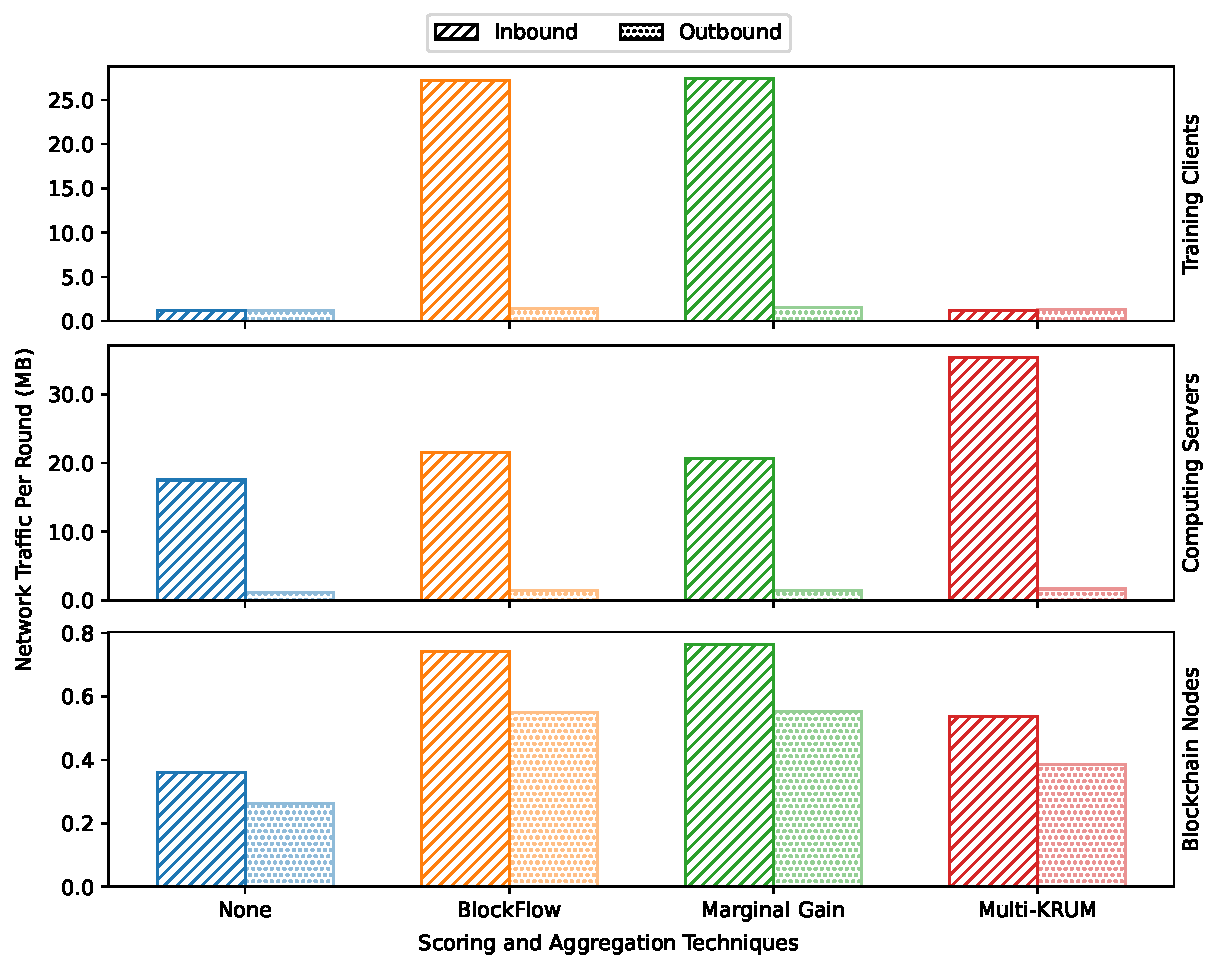
\includegraphics[width=0.8\textwidth]{graphics/04_scoring_net.pdf}
    \caption{Network Traffic Per Round Per Scoring technique}
    \label{fig:net_participants}
\end{figure}

\section{Computation Costs}

\begin{figure}[!hpt]
    \centering
    \centering
    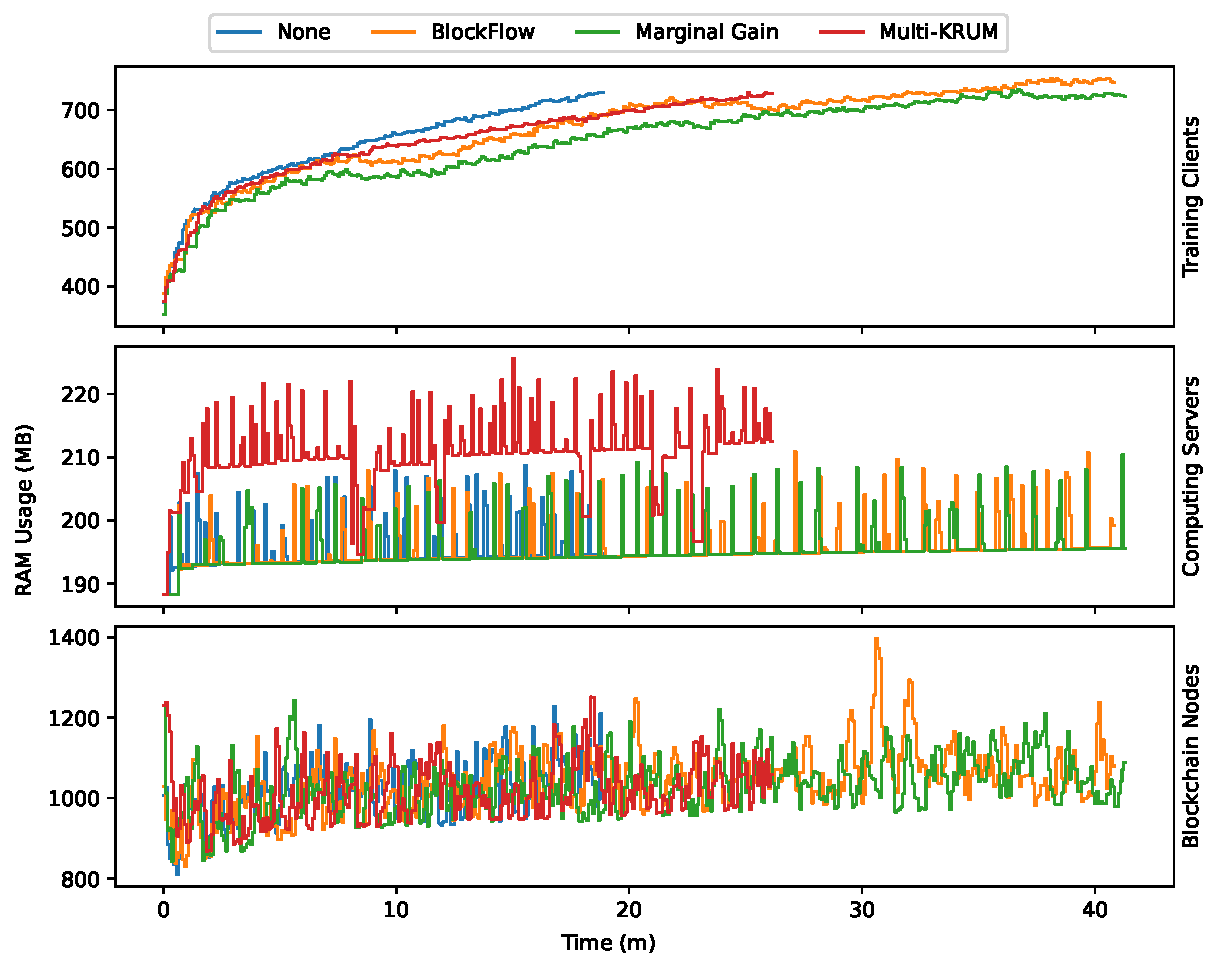
\includegraphics[width=0.8\textwidth]{graphics/04_scoring_ram.pdf}
    \caption{RAM Usage Per Scoring technique}
    \label{fig:ram_scoring}
\end{figure}

\begin{figure}[!hpb]
    \centering
    \centering
    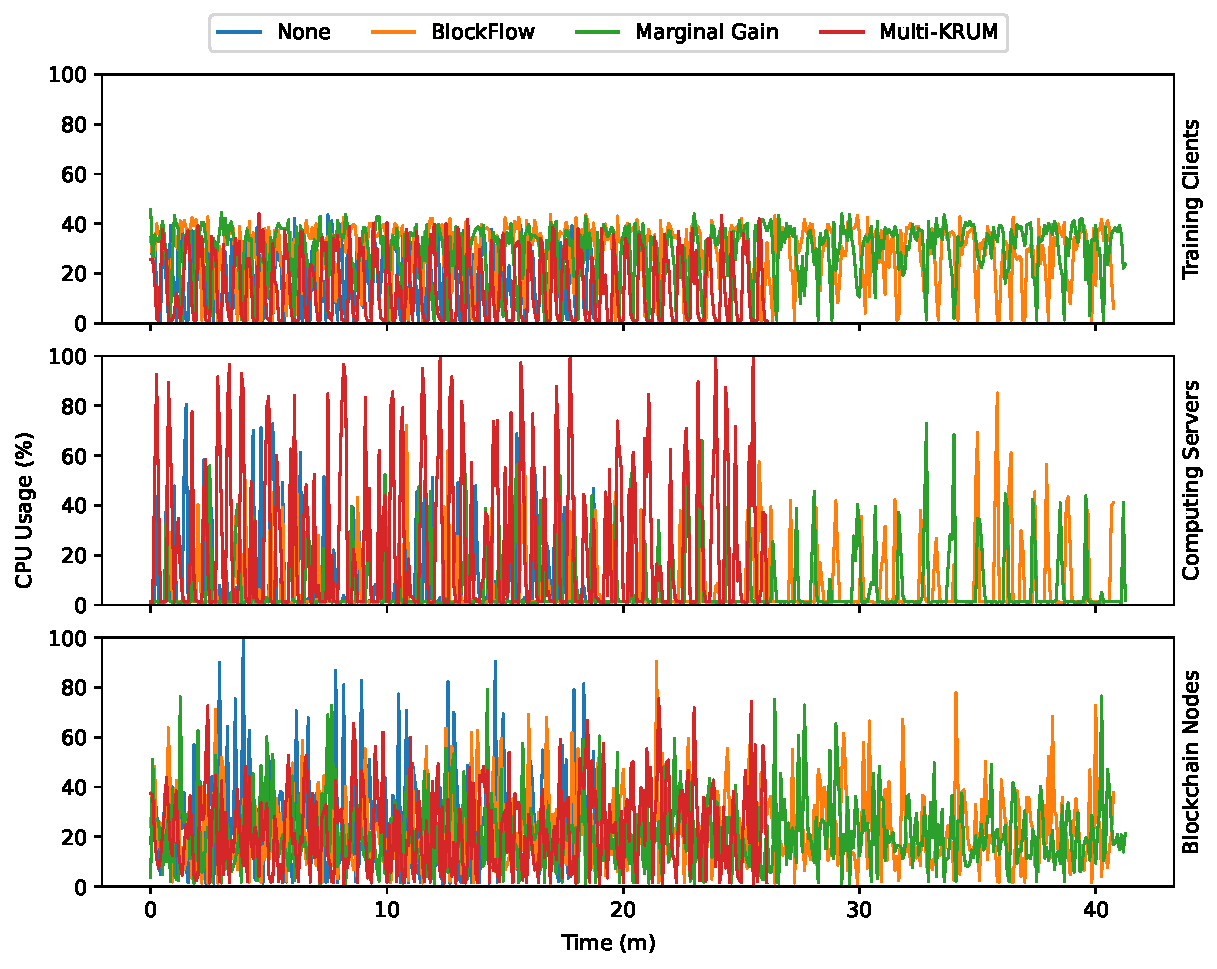
\includegraphics[width=0.8\textwidth]{graphics/04_scoring_cpu.pdf}
    \caption{CPU Usage Per Scoring technique}
    \label{fig:cpu_scoring}
\end{figure}

\section{Conclusions}

